\documentclass[a4paper,12pt, titlepage]{article}
\usepackage{amssymb,amsthm,amsmath}
\usepackage[finnish]{babel}
\usepackage[T1]{fontenc}
\usepackage[utf8]{inputenc}
\usepackage{graphicx}
\linespread{1.24}
\sloppy

\title{Tietokantasovellus \\ Dokumentaatio}
\author{Andreas Niskanen}
\date{\today}

\begin{document}

\maketitle

\tableofcontents

\newpage

\section{Johdanto}

Kisällikursseilla opiskelijat palauttavat viikoittain harjoitustehtäviä,
joista he voivat ansaita lisäpisteitä kurssisuoritukseen. Tehtäviä on
kahdenlaisia. Tähtitehtävät tarkistetaan, ja niistä saa pisteitä vain
silloin, kun tehtävä on tehty oikein. Tehtäviä saa kuitenkin korjata ja
palauttaa uudelleen. Tähdettömiä tehtäviä ei sen sijaan tarkisteta.\\
Tämä käytäntö vaatii toimiakseen pistekirjanpitojärjestelmän, jonka avulla
ohjaajat voivat kirjata opiskelijan palauttamia tehtäviä ja näiden korjauksia
mahdollisimman sujuvasti. Ohjaajan tulee myös nähdä opiskelijan palauttamat
tehtävät sopivassa muodossa ja muokata näitä tarpeen mukaan.\\
Kurssin opettajan vastuulla on lisätä järjestelmään kursseja ja poistaa
niitä järjestelmästä, sekä lisätä kullekin kurssille harjoitustehtäviä ja
hyväksyä ohjaajia, joilla on oikeudet muokata vain oman kurssin palautuksia.
Lisäksi opettajat tarvitsevat tiettyjä tilastollisia tunnuslukuja (esimerkiksi
palautettujen tehtävien määristä), jotka tulee näkyä kunkin kurssin yhteydessä.\\
Kyseinen pistekirjanpitojärjestelmä toteutetaan tietojenkäsittelytieteen
laitoksen users-palvelimelle käyttäen PostgreSQL-tietokantapalvelinta.
Palvelimen puolella käytetään PHP-ohjelmointikieltä, jonka avulla haetaan
tarvittava data tietokannasta ja tarjotaan REST-rajapinta selaimen puolella
käytettävän AngularJS-ohjelmistokehyksen käytettäväksi.

\newpage

\section{Käyttötapaukset}

\subsection{Käyttötapauskaavio}

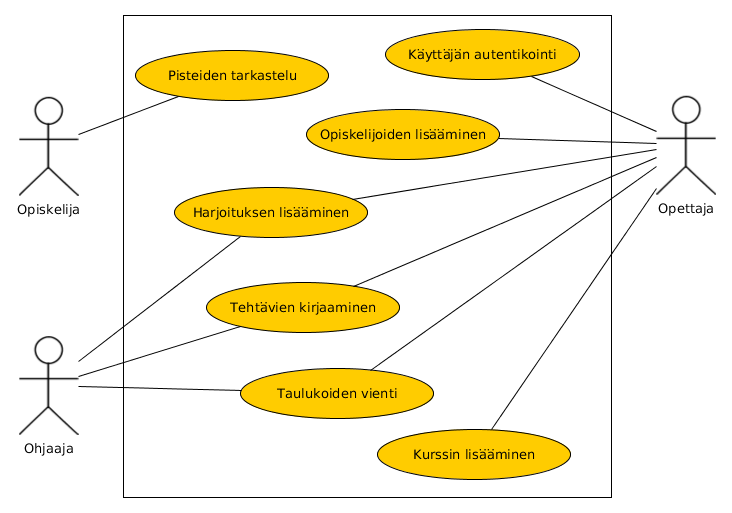
\includegraphics[scale=0.75]{kayttotapauskaavio}

\subsection{Käyttäjät}

\begin{description}
	\item[Ohjaaja] \hfill \\
	Ohjaajalla tarkoitetaan järjestelmään rekisteröitynyttä käyttäjää,
	jonka rekisteröityminen on hyväksytty opettajan toimesta.
	\item[Opettaja] \hfill \\
	Opettaja on rekisteröinyt ja autentikoitu käyttäjä, jonka vastuulla
	ovat omat kurssit ja harjoitustehtävät.
\end{description}

\subsection{Käyttötapauskuvaukset}

\begin{description}
	\item[Ohjaajan käyttötapaukset] \hfill \\
	\begin{description}
		\item[Tehtävien kirjaaminen] \hfill \\
		Ohjaajan tehtävänä on kirjata järjestelmään oman kurssin tehtäviä.
		Ohjaajan tulee myös tarvittaessa pystyä katsomaan ja muokkaamaan
		jo kirjattuja opiskelijan harjoituksen tehtäviä.
		\item[Muut käyttötapaukset:] rekisteröityminen, kirjautuminen
	\end{description}
	\item[Opettajan käyttötapaukset] \hfill \\
	\begin{description}
		\item[Ohjaajan autentikointi] \hfill \\
		Kun ohjaaja rekisteröityy järjestelmään tietyn kurssin ohjaajaksi,
		kurssin vastuuopettajan tulee vahvistaa ohjaajan käyttäjä.
		\item[Kurssin lisääminen] \hfill \\
		Opettajan tehtäviin kuuluu lisätä järjestelmään omia kursseja.
		Opettaja pystyy tarvittaessa myös muokkaamaan ja poistamaan kursseja.
		\item[Opiskelijan lisääminen] \hfill \\
		Opettajan tehtäviin kuuluu myös lisätä omille kursseille opiskelijoita
		kurssitunnuksen mukaan. Opettaja pystyy tarvittaessa myös muokkaamaan
		ja poistamaan opiskelijoita.
		\item[Harjoituksen lisääminen] \hfill \\
		Opettajan tehtäviin kuuluu myös lisätä omille kursseille harjoituksia
		määrittelemällä tehtävien lukumäärä. Opettaja pystyy tarvittaessa
		myös muokkaamaan ja poistamaan harjoituksia.
		\item[Taulukoiden vienti] \hfill \\
		Opettaja pystyy tulostamaan järjestelmästä taulukkona tietyn kurssin
		kaikkien opiskelijoiden palautettujen tehtävien lukumäärät, esimerkiksi
		.csv-muodossa.
		\item[Muut käyttötapaukset:] rekisteröityminen, kirjautuminen
	\end{description}
\end{description}

\end{document}
